\chapter{Open Content}


\section{I primi tentativi}

La \textbf{GNU Free Documentation License} è partita all'inizio perché c'era la necessità di avere una \textbf{documentazione libera}. Per molto tempo la documentazione che accompagnava il software libero era sotto licenza GPL e lo stesso TLDP (The Linux Documentation Project) distribuiva la sua documentazione sotto GPL, semplicemente perché era quello che ``passava al convento'', ma non ha molto senso usare la GPL per della documentazione. Se per esempio i \textit{Promessi Sposi} fossero stati pubblicati sotto licenza GPL io potrei prendere i sorgenti e cambiare nella copertina il nome dell'autore: questo posso farlo tranquillamente senza problemi se sono sotto GPL. Ma questo è un problema perché c'è differenza tra protezione del software e protezione del contenuto testuale. La tutela dell'autore originale è importante. Per questo motivo la GNU Free Documentation License si è posta come obiettivo una documentazione che avesse:

\begin{itemize}

\item Libertà di modifica;
\item Tutele dei diritti morali dell'autore;
\item Gestione del problema legato alle copie non trasparenti; come nel caso della GPL si vuole far sì che se qualcuno modifica un prodotto che è sotto GFDL quello rimanga disponibile nei suoi sorgenti (ad esempio non posso redistribuire un documento come serie di immagini jpeg che non sono editabili) e che non limiti la libertà di terzi di modificare la documentazione;
\item Copia in grande quantità e non.

\end{itemize}

\section{Concetti fondamentali}

È una licenza che nasce per la \textbf{documentazione} (soprattutto del progetto GNU). Si sente la necessità di dare al prodotto la possibilità di avere una documentazione sempre aggiornata quando esso viene rilasciato. Se ad esempio attuo una modifica al programma è necessario modificare la documentazione che ci sta dietro. 

Le parti del documento da considerare sono:

\begin{itemize}

\item Il \textbf{titolo}; se io modifico un documento sotto GFDL devo mantenere l'autore originale nella copertina aggiungendo eventualmente il mio;
\item Il documento in sè e il suo \textbf{contenuto};
\item \textbf{Sezioni secondarie e invarianti}, come ad esempio le dediche che possono essere modificate solamente mantenendo inalterato il tono. Le sezioni invarianti non possono assolutamente essere modificate ma devono essere al di fuori dell'argomento principale del documento;
\item \textbf{Testi di copertina}; posso modificare la copertina ma devo dichiararmi editore di quella versione;
\item \textbf{Storia del documento}, devo tenere traccia di tutte le modifiche e scriverle in una sezione del documento (esempio sezione Diario delle Modifiche);
\item La \textbf{licenza} dev'essere mantenuta e riportata nel documento.

\end{itemize}

Per quanto riguarda le copie trasparenti ci sono distinzioni per chi distribuisce sotto piccola quantità e grande quantità. In particolare se io voglio pubblicare un documento sul mio sito devo renderlo accessibile. Inoltre non devo aggiungere delle \textbf{restrizioni tecnologiche} che impediscano la modifica. 

Esiste tutta una serie di restrizioni per quanto riguarda la redistribuzione di \textbf{copie senza modifiche}:

\begin{itemize}

\item Mantenimento della licenza;
\item Nessuna misura tecnologica di restrizione;
\item Permettere di esibire la copia in pubblico;
\item Per quanto riguarda le redistribuzioni voluminose:
	\begin{itemize}

	\item Obbligo di identificarsi come autore;
	\item Obbligo di mantenere titoli e testi di copertina;
	\item Obbligo di distribuire una sorgente trasparente.

	\end{itemize}

\end{itemize}

Per quanto riguarda la redistribuzione di \textbf{copie modificate}:

\begin{itemize}

\item Devo modificare il titolo, in questo modo identifico il mio prodotto come qualcosa di diverso;
\item Indicazione degli autori delle modifiche e del documento originale;
\item Rimozione e/o aggiunta dei ``riconoscimenti'';
\item Aggiornamento della sezione cronologia;
\item Preservazione degli invarianti;
\item Preservazione della versione trasparente;
\item Preservazione e/o aggiunta dei testi di copertina.

\end{itemize}

Esistono anche tutta una serie di paragrafi di questa licenza che parlano essenzialmente dell'\textbf{unione di documenti}, delle collezioni e aggregati e delle \textbf{traduzioni} dei documenti. Per quanto riguarda le unioni di più documenti è necessario:

\begin{itemize}

\item Disambiguare tutte le parti;
\item Mantenere una licenza;
\item Rimuovere i riconoscimenti.

\end{itemize}

Un caso particolare è quando si tratta delle traduzioni: la traduzione è comunque considerata una modifica e in questo caso è necessario conservare la licenza e allo stesso tempo conservare gli invarianti. In questo modo si da garanzia all'autore che la sua opera non possa venire mal interpretata perché io potrei tradurla in maniera non appropriata (scritta male o con ambiguità). È possibile in ogni caso prendere accordi con l'autore.

\section{Il fallimento del copyright}

C'è stato un cambiamento enorme per quanto riguarda i tipi di diritti associati agli utenti e agli sviluppatori del software. 

\section{Gli anni d'oro della proprietà intellettuale}
\subsection{Il caso Nation - Ford}

Il presidente Gerald Ford scrisse una biografia includendo un anedotto sulla sua decisione di perdonare Richard Nixon. 
Ford aveva concesso sotto licenza i suoi diritti di pubblicazione alla Harper\&Row con un contratto per pubblicare un estratto delle memorie sul magazine Time. 
Invece, la rivista The Nation pubblicò dalle 300 alle 400 citazioni letterali direttamente dal libro di 500 pagine senza il permesso né di Ford, né della Harper\&Row né del Time.
Vista questa pubblicazione anticipata, il Time si tirò indietro dal contratto (il che era permesso da una clausola) e la Harper\&Row intentò una causa legale contro The Nation.\\

The Nation affermò che essendo Ford un personaggio pubblico e che le informazioni da lui divulgate fossero di vitale importanza la pubblicazione ricadesse sotto il fair use.\\

Un primo verdetto diede ragione alla Harper\&Row, ma uno successivo
della corte d'appello ribaltò la sentenza a favore di The Nation. Harper\&Row ricorse alla corte suprema, la quale ribaltò di nuovo il
verdetto, stabilendo che il fair use non è una difesa in caso di  
pre-pubblicazione e non permette l'appropriazione commerciale del 
lavoro di un famoso personaggio politico semplicemente 
a causa del pubblico interesse nell'apprendere informazioni su una
figura politica di un evento storico.\\

\begin{sloppypar}\tolerance=9999
\url{https://en.wikipedia.org/wiki/Harper_%26_Row_v._Nation_Enterprises}
\end{sloppypar}

\subsection{I ruoli di Kastenmeier e Schrader}

Robert Kastenmeier fu un politico americano membro del partito democratico. 
Dorothy Schrader fu consigliere generale per il Copyright Office degli Stati Uniti entrambi diedero un significativo contributo al Copyright Act del 1976.

\section{I prodromi della crisi}

Con l'avanzare di internet negli anni '90, il boom delle vendite di apparecchi elettronici e i film su videocassette si ha una contrapposizione tra utenti e lobby pro proprietà intellettuale che si fanno ancora più aggressive, arrivando a brevettare pressoché tutto (persino forme di vita come semi per l'agricoltura).

Dal punto di vista del software nello stesso periodo nasce l'EULA (\textit{End-User Licence Agreement}), un contratto tra il fornitore di un programma software e l'utente finale. Tale contratto assegna la licenza d'uso del programma all'utente nei termini stabiliti dal contratto stesso e nel 1990 nasce EFF (\textit{Electronic Frontier Foundation}) un'organizzazione internazionale non profit di avvocati e legali rivolta alla tutela dei diritti digitali e della libertà di parola nel contesto dell'odierna era digitale e il \textit{Berkman Center} un'istituto dell'università di Harvard dedicato allo studio e alla comprensione del Cyberspazio definendo e studiando norme, dinamiche e standard \url{https://cyber.law.harvard.edu/}

Tornando ai brevetti, nel 1999 Amazon arrivò a brevettare negli USA gli acquisti One-click (brevetto rifiutato nell'Unione Europea a causa di un mancato processo inventivo).

Negli anni '90 fece molto discutere il caso \textit{SEGA - Accolade}. Accolade casa produttrice e rivenditore di videogiochi, disassemblò tramite tecniche di Reverse Engineering alcuni giochi per la console Genesis di SEGA, in modo da poter pubblicare giochi compatibili per la console di SEGA senza il loro consenso. Il caso fece molto parlare di se visto che riguardava vari aspetti controversi come il copyright, l'uso permissivo di marchi e il fair use applicato al codice.
Nel 1992 SEGA vinse e Accolade fu costretta ad interrompere la produzione di giochi compatibili e a ritirare le copie dal mercato, Accolade ricorse in appello e il 28 agosto 1992 vinse (anche a seguito di forti pressioni da varie associazioni e del clamore mediatico del caso), quando la corte d'appello stabilì che la decompilazione ricadeva nel fair-use e condannò per altri motivi SEGA al pagamento di tutte le spese processuali. Alla fine le due compagnie trovarono un accordo conveniente ad entrambe. Il caso servì a stabilire che i principi funzionali del software non possono essere protetti da diritti d'autore (non e' possibile brevettare un algoritmo) e la corte incoraggiò la copia di software protetto per l'esplorazione di funzionalità non protette.\\

Altro evento importante fu l'approvazione da parte dell'amministrazione Clinton del \textit{National Information Infrastructure (NII)} un insieme di regole atte a costruire reti di comunicazione, servizi interattivi, hardware e software interattivo, per rendere disponibile sia al settore pubblico che privato una marea di informazione senza favorire un'azienda sull'altra. Purtroppo vennero anche introdotte ulteriori restrizioni, come la rimozione dei diritti di prima vendita e il DRM.

\section{Il movimento degli accademici}

Molti accademici nel mondo legale come Peter Jaszi e Lawrence Lessig iniziarono ad approfondire la questione legale attorno alla libertà d'espressione, il fair use e il copyright. In particolare Peter Jaszi fondò nel 1995 la \textit{Digital Future Coalition (DFC)} , un'organizzazione legale americana volta a trovare un giusto equilibrio tra salvaguardia della proprietà intellettuale e il libero accesso alla cultura e all'informazione. In particolare la DFC si oppose al white paper di Bruce Lehman in merito al NII e alle sue misure restrittive e al DMCA del 1998. Attualmente la DFC conta 42 altri enti e associazioni aderenti.\\

Nel 1994 venne pubblicato da John Perry Barlow \textit{The Economy of Ideas}, un articolo provocante qui riassunto in quattro punti:
\begin{itemize}
\item Le leggi sul copyright non si adattano bene a proprietà che possono essere infinitamente riprodotte e distribuite istantaneamente.
\item Le opere assumono valore nella trasmissione, l'informazione assume importanza se condivisa.
\item I beni intellettuali diventano sempre più prominenti ma proteggerne la proprietà è sempre più difficile.
\item Indifferenza sociale nei confronti della pirateria.
\end{itemize}
Sempre lo stesso autore pubblicherà nel 1996 un altro famoso manifesto \textit{La dichiarazione d'indipendenza del Cyber spazio}

Insomma a fine anni '90 vengono gettate le basi per licenze permissive, Authorship collettive (come wikipedia) e il dominio pubblico viene visto come una fonte di crescita, personale e sociale.

\section{Mickey Mouse Protection Art}

Nel 1998 venne approvato il \textit{Sonny Bono Copyright
Extension Act (SBCEA)} che estese di 20 anni i termini di protezione per le opere registrate dopo il 1923 negli USA. Il Sonny Bono Act prende il nome da un cantante che la appoggiò fortemente (salvo poi mai vederla approvata, visto che morì prima). La legge è anche conosciuta con il nome Mickey Mouse Protection Act, dal momento che la Disney ebbe un ruolo significativo nelle azioni di lobbismo per approvare la legge. Ogni volta che i diritti inerenti il personaggio di Topolino stanno per scadere, puntualmente viene approvata una legge per estendere la durata del copyright, come mostrato dal seguente grafico:

\begin{figure}[htbp]
\centering
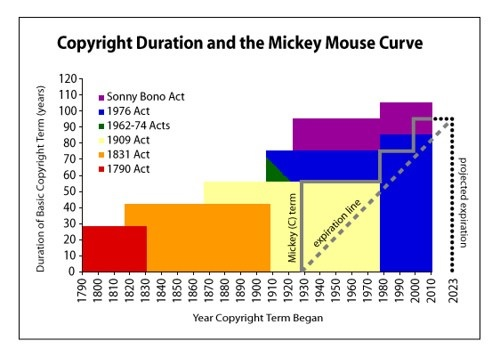
\includegraphics[width=50mm]{images/MM_copyright_graph}
\caption{Leggi sull'estensione del copyright e Topolino}
\end{figure}

\section{Eldred vs Reno}

Eric Eldred aveva fondato la Eldritch Press, un sito e casa editrice che pubblicava opere divenute di dominio pubblico appena scadevano i diritti d'autore, con l'approvazione del Sonny Bonno Act divenne impossibile proseguire il lavoro per le opere pubblicate dopo il 1922. \\

La sua storia si intrecciò a quella di Lessig. Lessig, giovane avvocato e attivista politico era interessato alla legge come strumento di cambiamento politico e all'impatto della società sulla legge. I due strinsero quindi un patto che sfociò nel dibattimento Eldred vs Reno con l'obiettivo di denunciare l'incostituzionalità del SBCEA, purtroppo i due persero davanti alla corte suprema nel 2003, la quale stabilì che l'estensione retroattiva di vent'anni del copyright esistente non violava la clausola del diritto d'autore o il Primo emendamento della Costituzione degli Stati Uniti d'America.  Il caso ebbe comunque un'ampia risonanza e fu il primo esperimento di \textit{openlaw} con tanto di newsletter e forum nei quali l'opinione pubblica veniva informata dello svolgersi del processo e delle varie iniziative legali a tutela del dominio pubblico.\\

Se Topolino smuoveva interessi economici troppo forti i due decisero di dedicarsi ad opere minori creando un movimento tecnico - legale puntando sula copyright conservancy, portando quindi alla nascita di Creative Commons.

\section{Creative Commons}
La nascita di Creative Commons passò prima per vari step

\begin{itemize}
\item 1999: nasce Copyright Commons diretto da Jennifer Love e Ashley Morgan, una newsletter mensile sul caso Eldred vs Reno e varie news sul public domain

\item Nasce la Campagna Counter Copyright (CC): Ponendo l'icona CC (il counter-copyright) alla fine dell'opera, l'autore segnala agli altri che permette di usare, modificare, adattare e ridistribuire il suo lavoro. Il Counter Copyright non è un rimpiazzo al copyright attuale, è solo un segnale che l'autore permette agli altri di condividere il suo lavoro. 
Però il Counter Copyright strappò via al copyright l'esclusività di fornire e autorizzare altre persone per l'uso di un'opera per le loro opere creative.

\item 1999: Napster incontra i talk di Lessig

\item 2000 - Abelson ha l'idea di  una fondazione che accetti donazioni di opere

\item 2001: viene fondato Creative Commons, un'organizzazione statunitense non profit dedicata ad ampliare la gamma di opere creative disponibili alla condivisione e all'utilizzo pubblico in maniera legale. Rende possibile il riuso creativo di opere dell'ingegno altrui nel pieno rispetto delle leggi esistenti.
Il nome nasce da un gioco di parole sulla “tragedia dei beni comuni”
di Garret Hardin \url{https://it.wikipedia.org/wiki/Tragedia_dei_beni_comuni}

\item 2003: nasce il distaccamento italiano
\end{itemize}

\subsection{Obiettivi}
\begin{itemize}
\item Promuovere la diffusione di un modello “alcuni diritti riservati”

\item Tutelare il marchio “Creative Commons”

\item Creazione di appropriati strumenti legali e tecnologici
\end{itemize}

Il tutto senza essere né un ente pubblico, né organismo per la raccolta dei diritti d'autore e soprattutto senza offrire servizi di consulenza legale.

\section{Le licenze Creative Commons}

Creative Commons permette agli utenti di rilasciare il loro lavoro scegliendo tra varie licenze pensate per opere creative (non software) disponibili per 52 sistemi giuridici permettendo di 

\begin{itemize}
\item Preservare delle note di licenza
\item Copiare e distribuire l'opera
\item Esibire l'opera o convertirla di formato
\end{itemize}

E vientando l'uso di restrizioni tecnologiche.

Ogni licenza si compone di tre parti:
\begin{itemize}
\item \textbf{Commons Deed}: una sintesi del contratto comprensibile a chiunque tramite un breve riassunto e dei simboli facilmente comprensibili e riconoscibili. I 4 simboli combinabili tra loro sono:

\begin{figure}[htbp]
\centering
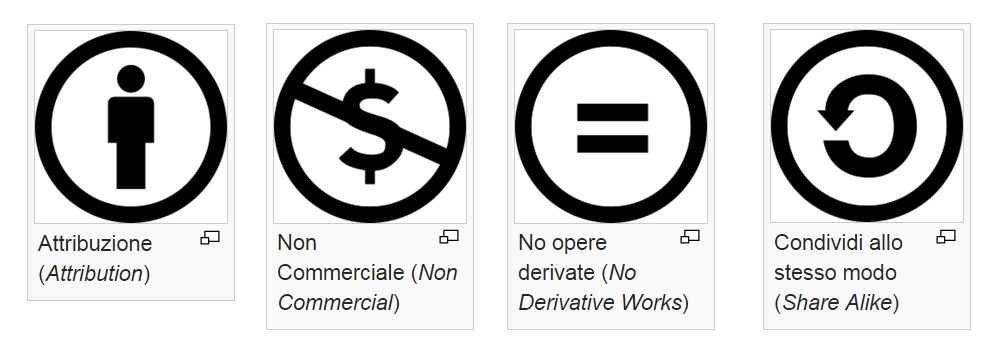
\includegraphics[width=50mm]{images/CC_Deed}
\caption{Le quattro clausole base delle Licenze CC}
\end{figure}

Condividi allo stesso modo (Share Alike - SA) e No Opere derivate (ND) non possono essere combinati tra loro

\item \textbf{Legal Code}: l’intero contratto espresso in linguaggio tecnico-giuridico in base al paese scelto. E' la licenza vera è propria.
\item \textbf{Digital Code}: Metadati che descrivono gli elementi chiave della licenza, applicando all'opera un codice che la rende ricercabile dai motori di ricerca abilitati.
\end{itemize}

\subsection{Le sei licenze}
Le sei licenze CC sono:

\begin{wrapfigure}{L}{0.15\textwidth}
    
\includegraphics[width=20mm]{images/cc_by}
\end{wrapfigure}

\noindent \textbf{Attribuzione CC BY} Questa licenza permette a terzi di distribuire, modificare, ottimizzare ed utilizzare l' opera come base, anche commercialmente, fino a che sia riconosciuto il credito per la creazione originale all'autore. Questa è la più accomodante delle licenze offerte ed è raccomandata per la diffusione e l'uso massimo di materiali coperti da licenza.\\
\begin{wrapfigure}{L}{0.15\textwidth}
    
\includegraphics[width=20mm]{images/cc_by_sa}
\end{wrapfigure}

\noindent \textbf{Attribuzione - Condividi allo stesso modo CC BY-SA} Estende la precedente permettendo la redistribuzione anche a scopo commerciale e autorizza le loro nuove creazioni con i medesimi termini. Questa licenza è spesso comparata con le licenze usate dai software opensource e gratuite "copyleft". Tutte le opere basate sull'originale porteranno la stessa licenza, quindi tutte le derivate permetteranno anche un uso commerciale. Questa è la licenza usata da Wikipedia, ed è consigliata per materiali che potrebbero beneficiare dell'incorporazione di contenuti da progetti come Wikipedia e similari.\\

\begin{wrapfigure}{L}{0.15\textwidth}
    
\includegraphics[width=20mm]{images/cc_by_nd}
\end{wrapfigure}

\noindent \textbf{Attribuzione - Non opere derivate CC BY-ND} Questa licenza permette la ridistribuzione, commerciale e non, fintanto che viene trasmessa intera ed invariata, dando credito all'autore. Non permette tuttavia la creazione di opere derivate.\\

\begin{wrapfigure}{L}{0.15\textwidth}
    
\includegraphics[width=20mm]{images/cc_by_nc}
\end{wrapfigure}

\noindent \textbf{Attribuzione - Non commerciale CC BY-NC} Questa licenza permette a terzi di modificare, ottimizzare ed utilizzare l' opera come base per altre non commerciali, anche le opere derivate dovranno essere non commerciali.\\

\begin{wrapfigure}{L}{0.15\textwidth}
    
\includegraphics[width=20mm]{images/cc_by_nc_sa}
\end{wrapfigure}

\noindent \textbf{Attribuzione - Non commerciale - Condividi allo stesso modo CC BY-NC-SA} Questa licenza permette a terzi di modificare, redistribuire, ottimizzare ed utilizzare l'opera come base non commerciale, fino a che riconoscano i crediti all'autore e licenzino le loro nuove creazioni mediante i medesimi termini.\\

\begin{wrapfigure}{L}{0.15\textwidth}
    
\includegraphics[width=20mm]{images/cc_by_nc_nd}
\end{wrapfigure}

\noindent \textbf{Attribuzione - Non commerciale - Non opere derivate 
CC BY-NC-ND} Questa licenza è la più restrittiva delle sei principali, permettendo a terzi soltanto di scaricare le opere e condividerle ad altri fino a che riconoscano i giusti crediti, ma non possono cambiarle in nessun modo od utilizzarle commercialmente.\\

Le licenze sono pensate anche per trattare lavori collettivi (dove l'opera è parte di una più ampia) e opere derivate e permettono la distribuzione della licenza e delle clausole di salvaguardia anche attraverso url.\\

Devono includere:
\begin{itemize}
\item La citazione dell'autore originario, rimovibile su richiesta del licenziante
\item Titolo dell'opera originaria
\item Se possibile url associato all'opera
\item Uso dell'opera
\end{itemize}

\section{Altri strumenti}

Creative Commons oltre alle licenze sopra descritte fornisce anche altri strumenti utili agli autori:\\

\begin{wrapfigure}{L}{0.15\textwidth}
    
\includegraphics[width=20mm]{images/CC0}
\end{wrapfigure}

\noindent \textbf{CC0} Un'alternativa al dominio pubblico, il detentore dei diritti d'autore può rinunciare a tutti i suoi interessi sulla sua opera.\\ \\

\begin{wrapfigure}{L}{0.15\textwidth}
    
\includegraphics[width=20mm]{images/cc_PD}
\end{wrapfigure}

\noindent \textbf{Marchio di pubblico dominio} Per marcare opere libere da restrizioni di copyright\\

\textbf{CC plus (CC+)} Un protocollo RDF per esprimere licenze alternative, è possibile combinare le licenze CC con altre separate ed indipendenti che diano più diritti, senza però modificare il legal code originale.\\

\textbf{Founders Copyright} Non più supportato, permetteva agli autori di detenere i diritti per l'opera per 14 anni e poi questa diveniva di pubblico dominio. Si ispirava alle leggi sul diritto d'autore in vigore nel 1790, senza cambiare nessuna legge in vigore aiutava i detentori di diritti che ritenessero troppo lungo il periodo di 70 anni, di rilasciare le opere dopo un periodo molto più corto.

\subsection{Link utili}

E' possibile scegliere una licenza CC all'indirizzo: \\

\url{https://creativecommons.org/choose/}\\

Mentre per usare CC0 il link è il seguente: \\

\url{https://creativecommons.org/choose/zero/waiver}\\

compilando un semplice form online.\\

E' inoltre possibile ricercare opere poste sotto licenze CC al link \\

\url{http://search.creativecommons.org/}.\\

\section{Scarichiamoli}

Scarichiamoli è un progetto creato all'interno di Creative Commons
Italia: \\

\url{http://www.scarichiamoli.org/main.php} \\

Le opere di ingegno finanziate a fondo perduto con soldi pubblici dovrebbero essere:

\begin{itemize}
\item Pubblicamente accessibili: facilmente reperibili su Internet
\item Universalmente accessibili: accessibili anche per i diversamente abili
\item Liberamente fruibili: non occorre pagare per: leggere un testo, vedere un'immagine, ascoltare una musica
\item legalmente fruibili: (l'utente è certo di poter scaricare un file nella piena legalità)
\item ottimamente fruibili (qualità digitale idonea a garantire una buona visualizzazione e/o un buon ascolto)
\end{itemize}